\documentclass[geometry-lectures-19.tex]{subfiles}

\begin{document}



\subsection{Cohomology groups}
Given a simplicial complex $K$ and its chain group $C_k(K)$, we can define the \textbf{cochain group}
$$
C^k(K)=\{ f:C_k(K)\to \bZ, \ \ \textrm{homomorphism}\}
$$
In addition, we can define a \textbf{coboundary map} $\delta:C^k(K)\to C^{k+1}(K)$ as $\delta f(c)=f(\partial c)$ were $c\in C_{k+1}(K)$. It is easy to see $\delta\cdot \delta =0$, so that we obtain the cochain complex
\[
 0\xleftarrow{\delta^{n+1}}C^n\xleftarrow{\delta^{n}}C^{n-1}\xleftarrow{\delta^{n-1}}\cdots \xleftarrow{\delta^{2}} C^1\xleftarrow{\delta^{1}}C^0\xleftarrow{\delta^{0}}0
\]

We can define \textbf{cocycle} $Z^k(K)=\Ker\delta^k$ and \textbf{coboundary} $B^k(K)=\Im\delta^{k-1}$. The cohomology group of $K$ is defined by
$$
H^k(K;\bZ)=Z^k(K)/B^k(K)~.
$$
There exists bilinear map
$$
H_k(K;\bZ)\otimes H^k(K;\bZ)\to \bZ; ([c],[f])\mapsto f(c)
$$
which is well defined.

In a similar fashion, one can also define the cohomology group with $\bR$-coefficient. In fact, the cohomology group with $\bR$-coefficient is dual to the homology group $$H^{q}(C^{\bullet}, \mathbb{R})=\left(H_{q}\left(C_{\bullet}, \mathbb{R}\right)\right)^{*}~.$$
The case of the $\bZ$-coefficient is not so straightforward. (Can you find an example in which the cohomology groups are not dual of the homology groups?) We need the universal coefficient theorem for $H^{q}(C^{*}, \mathbb{Z})$, for which we refer to \cite[Theorem 3.2]{hatcher2005algebraic}.

\bthm[de Rham]
Let $M$ be a smooth manifold and $|K|\to M$ be its triangulation. Then, we have an isomorphism
$$
H^\bullet_{dR}(M)\cong H^\bullet(K;\bR)~.
$$
\ethm
A proof requires \v{C}ech cohomology, which is given in \cite{warner2013foundations,morita2001geometry}. As in the wedge product of the de Rham cohomology group, the simplicial cohomology group is endowed with product structure, called \textbf{cup product}.  For cochains \(\varphi \in C^{k}(X ; R)\) and \(\psi \in C^{\ell}(K;R)\) with $R$-coefficient ($R=\bZ_m,\bZ,\bR$), the cup product \(\varphi \cup \psi \in C^{k+\ell}(K;R)\) is the cochain whose paring with a simplex \(\sigma =\langle a_0,a_1,\ldots,a_{k+\ell}\langle\) is given by the formula
$$(\varphi \cup \psi)(\sigma)=\varphi(\langle a_{0}, \ldots, a_{k}\rangle ) \psi (\langle a_{k}, \ldots, a_{k+\ell}\rangle )$$
where the RHS is given by the product in the ring $R$. As a result, $(H^\bullet(K;R),\cup)$ is callled the cohomology ring of $K$.

In fact, there is an important relation between homology group and cohomology group of a oriented connected closed manifold $M$. A $k$-dimensional oriented submanifold $N\subset M$ without boundary indeed represents a generator $[N]\in H_k(M;\bR)$.  There exists $\eta\in H^{n-k}(M;\bR)$ such that
$$
\int_N \omega =\int_M\omega\wedge \eta
$$
for any $\omega\in H^k(M;\bR)$.

\bthm[Poincar\'e duality]
Let $M$ be an $n$-dimensional oriented connected closed manifold. Then, we have an isomorphism
$$
\vartheta: H_{k}(M;\bR)\cong H^{n-k}(M;\bR); [N]\mapsto \eta~.
$$
\ethm
In fact, the Poincar\'e duality holds any ring coefficient $R=\bZ_m,\bZ,\bR$.
Using this isomorphism, one can define an \textbf{intersection number} $[N_1]\cdot [N_2]$ for $[N_1]\in H^k(M;\bR)$ and $[N_2]\in H^{n-k}(M;\bR)$.
$$
[N_1]\cdot [N_2]:=\int_M \eta_1\wedge \eta_2
$$
where $\vartheta(N_i) =\eta_i$.



\subsection{Lefschetz fixed point theorem and Poincar\'e-Hopf theorem}\label{sec:Lefschetz}
Let $M$ and $N$ be $n$-dimensional smooth oriented connected closed manifolds.
A smooth map $f:M\to N$ induces an homomorphism $f_*:H_\bullet(M;\bZ)\to H_\bullet(N;\bZ)$. In particular, we define \textbf{mapping degree} of $f$ by
$$
 f_*([M]):=(\deg f) [N]~.
$$
In the language of cohomology group, we can define
$$
\deg f:= \frac{\int_Mf^* \omega} {\int_N\omega}
$$
where $\omega$ is the volume form of $N$.

Given two knots $K_1,K_2:S^1\to \bR^3$, we can define $F:K_1\times K_2\to S^2$ by
$$
F(p,q)=\frac{x_1-x_2}{|x_1-x_2|}
$$
Then, we define the \textbf{linking number} of $K_1$ and $K_2$ as
$$
Lk(K_1,K_2):=\deg F=\frac{1}{4\pi}\int_{K_1\times K_2} F^* \omega=\frac{1}{4\pi}\int_{K_1}dx_1^i \int_{K_2} dx_2^j \frac{(x_1-x_2)^k}{|x_1-x_2|^3}\epsilon_{ijk}
$$
where $\omega$ is the volume form of $S^2$.
\begin{figure}[ht]\centering
\includegraphics{pictures/linking}
\end{figure}

This number was first introduced by Gauss in the study of electromagnetism.  Biot-Savart law tells us that the magnetic field generated by electric current running on $K_1$ with unit strength is
$$
\vec{B}(\vec x)= \frac1{4\pi}\int_{K_1}  \frac{(\vec{x}-\vec {x_1}(t_1))^k\times \frac{d\vec {x_1}}{dt_1} }{|\vec x- \vec x_1|^3}dt_1
$$
Therefore, $Lk(K_1,K_2)$ is the energy which costs to move a magnetic monopole along $K_2$ under this magnetic field. Gauss has noticed that the integral always provides an integer however $K_1$ and $K_2$ are drawn. Moreover, this number stays invariant even though you deform $K_1$ and $K_2$!


Let $M$ be an $n$-dimensional smooth closed oriented manifold.
We assume that a map $f:M\to M$ has isolated fixed points $f(p)=p$. We define a map $h:S^{n-1}_\epsilon\to S^{n-1}$ by
$$
h(q)=\frac{q-f(q)}{|q-f(q)|}
$$
The index of $f$ at the fixed point $p$ is defined by
$$
\textrm{ind}_p f:=\deg h
$$
We define the \textbf{Lefschetz number} of $f$ as
  \[
    L(f) = \sum_{i \geq 0} (-1)^i \Tr(f_*:H_i(M;\bR) \to H_i(M;\bR)).
  \]

\bthm[Lefschetz fixed point theorem]
The Lefschetz number is the sum of indices over isolated fixed points
$$
 L(f)=\sum_{p} \textrm{ind}_p (f)
$$
\ethm


 The Lefschetz theorem can be interpreted from the viewpoint of intersection numbers. Given a smooth map $f:M \to M$, we can define a submanifold $\Gamma_f$ called the \textbf{graph} of $f$
$$
\Gamma_f=\{(x,f(x))\in M\times M\}~.
$$
For the identity map, the corresponding graph $\Gamma_{\textrm{id}}$ is called the diagonal submanifold of $M\times M$. Then, the Lefschetz number is given by an intersection number of $[\Gamma_f]$ and $[\Gamma_{\textrm{id}}]$ in $M\times M$
$$
L(f)=[\Gamma_f]\cdot [\Gamma_{\textrm{id}}]~.
$$
\begin{center}
  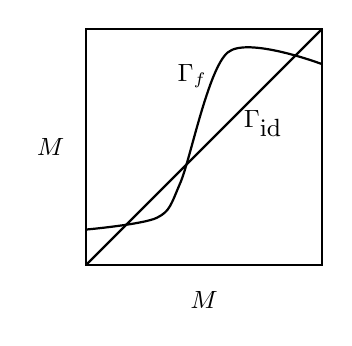
\begin{tikzpicture}[scale=1.5]
    \draw [thick] (0,0) -- (2,0) -- (2,2)--(0,2)--cycle;
        \draw [thick] (0,0)  -- (2,2);
        \draw [thick] plot [smooth] coordinates {(0,.3) (.6,.4) (.8,.7)(1.2,1.8) (2,1.7) };
        \node at (.9,1.6) {\small $\Gamma_f$};
        \node at (1.5,1.2) {\small $\Gamma_{\textrm{id}}$};
        \node at (1,-.3) {\small $M$};
                \node at (-.3,1) {\small $M$};
  \end{tikzpicture}
\end{center}



Let $X$ is a smooth vector field on $M$ and $\varphi_t$ is a flow generated by $X$. Then, the index of a zero point $p$ of $X$ is defined by
$$
\textrm{ind}_p (X) =\textrm{ind}_p(\varphi_t)~.
$$
Since the flow $\varphi_t$ is homotopic to the identity $\varphi_t\simeq \id$, $L(\varphi_t)$ is equal to the Euler characteristic.
$$
    L(\varphi_t) =\sum_{i \geq 0} (-1)^i \Tr(\id:H_i(M;\bR) \to H_i(M;\bR)).=\sum_{i \geq 0} (-1)^i \dim H_i(M;\bR) =\chi(M)
$$
Therefore, we obtain:
\bthm[Poincar\'e-Hopf theorem]
The Euler characteristics is the sum of indices over isolated fixed points
$$
\chi(M)=\sum_{p} \textrm{ind}_p (X)
$$
\ethm


\begin{minipage}[b]{6.5cm}
\includegraphics[width=5.5cm]{pictures/vector-fields}
\end{minipage}
\begin{minipage}[b]{8cm}
\includegraphics[width=8.5cm]{pictures/vector-field-indices}
\end{minipage}


This theorem was introduced in \S\ref{sec:Euler}. There is another important ``fixed point theorem'' due to Brouwer, which we delegate to \cite{milnor1965topology}.


























\section{Fundamental groups and Homotopy groups}




\subsection{Fundamental groups}


  A \textbf{path} in a topological space $M$ is a map $\gamma: I\to M$. If $\gamma(0) = x_0$ and $\gamma(1) = x_1$, we say $\gamma$ is a path from $x_0$ to $x_1$.  If $\gamma(0) = \gamma(1)$, then $\gamma$ is called a \textbf{loop} (based at $x_0$).  The idea of fundamental groups is to consider homotopy equivalence of loops at a fixed base point $x_0$

\bdefn[Fundamental group]
  Let $M$ be a topological space and $x_0 \in M$. The \textbf{fundamental group} of $M$ (based at $x_0$), denoted $\pi_1(M, x_0)$, is the set of homotopy classes of loops in $M$ based at $x_0$ (i.e.\ $\gamma(0) = \gamma(1) = x_0$). The group operations are defined as follows:

  We define a group multiplication by $[\gamma_0][\gamma_1] = [\gamma_0\cdot \gamma_1]$; inverses by $[\gamma]^{-1} = [\gamma^{-1}]$; and the identity as the constant map $e = [c_{x_0}]$.
\edefn



It is easy to see from the figure below that fundamental groups are independent of the choice of a base point. Therefore, it is often written as $\pi_1(M)$.
\begin{center}
  \begin{tikzpicture}
    \draw plot [smooth cycle] coordinates {(-2.4, -0.7) (0, -0.7) (1.4, -1) (2.6, -0.9) (2.8, 0.6) (0.6, 1.9) (-3.4, 0.8)};

    \node [circ] at (-2, 0.2) {};
    \node [anchor = south west] at (-2, 0.2) {$x_0$};
    \node [circ] at (1.5, 0.1) {};
    \node [above] at (1.5, 0.1) {$x_1$};

    \draw [->-=0.5] (-2.4, 0.2) circle [radius = 0.4];
    \draw [->-=0.5] (-2, 0.2) parabola bend (-0.25, 0) (1.5, 0.1) node [pos=0.5, below] {$u$};
    \draw [mred, ->-=0.3, ->-=0.7] (1.5, 0.1) -- (1.5, 0.2) parabola bend (-0.25, 0.1) (-2, 0.3) arc (14:346:0.4123) parabola bend (-0.25, -0.1) (1.5, 0) -- (1.5, 0.1);
  \end{tikzpicture}
\end{center}


Unlike homology goups, the fundamental groups are non-abeilan groups in general.
\bexample
Let us consider the space  $M=\bR^2\backslash \{p_1,p_2\}$ which is obtained by removing two points from the plane.
The fundamental group of $M$ is the free group  $\pi_1(M) = F(\{ a, b\})$ with the two generators. See Definition \ref{def:free-group}. It is easy to understand the free group on two generators by the \textbf{Cayley graph} below.
\eexample
\begin{figure}[h]\centering
  \begin{minipage}[b]{0.4\textwidth}
 \raisebox{1cm}{ \begin{tikzpicture}
    \draw (-1.5, 0) circle [radius=1.5];
    \draw (1.5, 0) circle [radius=1.5];
    \draw (-1.5, 0) circle [radius=.1];
    \draw (1.5, 0) circle [radius=.1];
    \node [circ] {};
    \node [left] at (-3, 0) {$a$};
    \node [right] at (3, 0) {$b$};
    \node [left] at (-1.5, 0) {$p_1$};
    \node [right] at (1.5, 0) {$p_2$};
    \draw [->] (3, 0.1) -- (3, 0.11);
    \draw [->] (-3, 0.1) -- (-3, 0.11);
    \node [right] {$x_0$};
\end{tikzpicture}}
\end{minipage}
\hspace{1cm}
\begin{minipage}[b]{0.4\textwidth}
  \begin{tikzpicture}[scale=0.5]
    \draw (-3, 0) -- (3, 0);
    \draw (0, -3) -- (0, 3);
    \foreach \x/\y/\rot in {3/0/0, 0/3/90, -3/0/180, 0/-3/270} {
      \begin{scope}[shift={(\x, \y)}, scale=0.5, rotate=\rot]
        \draw (0, 0) -- (3, 0);
        \draw (0, 3) -- (0, -3);
        \foreach \x/\y/\rot in {3/0/0, 0/3/90, 0/-3/270} {
          \begin{scope}[shift={(\x, \y)}, scale=0.5, rotate=\rot]
            \draw (0, 0) -- (3, 0);
            \draw (0, 3) -- (0, -3);
            \foreach \x/\y/\rot in {3/0/0, 0/3/90, 0/-3/270} {
              \begin{scope}[shift={(\x, \y)}, scale=0.5, rotate=\rot]
                \draw (0, 0) -- (3, 0);
                \draw (0, 3) -- (0, -3);
                \foreach \x/\y/\rot in {3/0/0, 0/3/90, 0/-3/270} {
                  \begin{scope}[shift={(\x, \y)}, scale=0.5, rotate=\rot]
                    \draw (0, 0) -- (3, 0);
                    \draw (0, 3) -- (0, -3);
                    \foreach \x/\y/\rot in {3/0/0, 0/3/90, 0/-3/270} {
                      \begin{scope}[shift={(\x, \y)}, scale=0.5, rotate=\rot]
                        \draw (0, 0) -- (3, 0);
                        \draw (0, 3) -- (0, -3);
                      \end{scope}
                    }
                  \end{scope}
                }
              \end{scope}
            }
          \end{scope}
        }
      \end{scope}
    }
    \node [circ] {};
    \node [anchor = south west] {$\widetilde{x}_0$};
    \draw [->] (1.7, 0) -- (1.71, 0);
    \node [above] at (1.5, 0) {$a$};
    \draw [->] (-1.3, 0) -- (-1.29, 0);
    \node [above] at (-1.5, 0) {$a$};

    \draw [->] (0, 1.7) -- (0, 1.71);
    \node [left] at (0, 1.5) {$b$};
    \draw [->] (0, -1.3) -- (0, -1.29);
    \node [left] at (0, -1.5) {$b$};

    \draw [->] (3.9, 0) -- (4, 0);
    \node [above] at (3.75, 0) {$a$};

    \draw [->] (3, 0.9) -- (3, 1);
    \node [left] at (3, 0.75) {$b$};
    \draw [->] (3, -0.5) -- (3, -0.4);
    \node [left] at (3, -0.75) {$b$};
  \end{tikzpicture}
\end{minipage}
\end{figure}

Usually, a fundamental group is presented as $\langle S\mid R\rangle$ by generators $S$ and the relations $R$. See Definition \ref{def:presentation}. As it can be easily read off from Figure \ref{fig:torus}, the fundamental group of a torus is
$$
\pi_1(T^2)\cong \langle a,b\mid aba^{-1}b^{-1}\rangle~.
$$




  A \textbf{based space} is a pair $(M, x_0)$ of a topological space $M$ and a \textbf{base point} $x_0\in M$. A \textbf{map of based spaces}
  \[
    f: (M, x_0) \to (N, y_0)
  \]
  is a continuous map $f: M\to N$ such that $f(x_0) = y_0$. A based map $f$ induces the group homomorphism
  \[
    f_* : \pi_1(M, x_0) \to \pi_1(N, y_0),
  \]
  defined by $[\gamma] \mapsto [f\circ \gamma]$. Thus, the induced homomorphisms are natural under compositions: For $\begin{tikzcd} (M, x_0) \ar[r, "f"] & (N, y_0) \ar[r, "k"] & (L, z_0) \end{tikzcd}$, we have $(k\circ h)_\ast = k_\ast\circ h_\ast$
  Moreover, if two based maps $f_0, f_1$ are homotopic $f_0 \simeq f_1$, then $(f_0)_\ast=(f_1)_\ast$.





\bthm
  If $f: M\to N$ is a homotopy equivalence, and $x_0 \in M$, then the induced map
  \[
    f_*: \pi_1(M, x_0) \to \pi_1(N, f(x_0)).
  \]
  is an isomorphism.
\ethm

\bexample
Let us denote the space obtained by joining two copies of $S^1$ at one point by $S^1 \vee S^1$. Then, it is homotopic to $\bR^2\backslash \{p_1,p_2\}$ so that the fundamental group is $\pi_1(S^1\vee S^1)\cong F(\{ a,b\})$.
\eexample
% \begin{proof}
%   Let $g: Y\to M$ be a homotopy inverse so that $f\circ g\simeq \id_N$ and $g\circ f\simeq \id_M$.
%   \begin{center}
%     \begin{tikzpicture}
%       \draw plot [smooth cycle] coordinates {(-3.7, -1.2) (-3.7, 0) (-4, 0.7) (-3.9, 1.3) (-2.4, 1.4) (-1.8, 0.3) (-2.2, -1.7)};
%       \draw plot [smooth cycle] coordinates {(1.3, -1.2) (1.3, 0) (0.7, 0.7) (0.6, 1.3) (2.6, 1.4) (3, 0.3) (2.8, -1.7)};
%
%       \node [circ] at (-3, 0.7) {};
%       \node [above] at (-3, 0.7) {$x_0$};
%       \node [above] at (-3, 1.6) {$M$};
%
%       \node [above] at (1.8, 1.6) {$N$};
%
%       \node [circ] at (1.8, 0.8) {};
%       \node [below] at (1.8, 0.8) {$f(x_0)$};
%
%       \node [circ] at (-3, -0.8) {};
%       \node [below] at (-3, -0.8) {$g\circ f(x_0)$};
%
%       \draw [decoration={snake}, decorate] (-3, 0.7) -- (-3, -0.8) node [right, pos=0.5] {$\eta$};
%
%       \draw [->] (-1.6, 1) parabola bend (-0.7, 1.3) (0.2, 1.2);
%       \node [above] at (-0.7, 1.3) {$f$};
%
%       \draw [->] (1, -1.1) parabola bend (-0.3, -1.3) (-1.6, -1);
%       \node [below] at (-0.3, -1.3) {$g$};
%     \end{tikzpicture}
%   \end{center}
%   We have no guarantee that $g\circ f(x_0) = x_0$, but we know that our homotopy $H'$ gives us $\eta = H'(x_0, \ph): x_0 \leadsto g\circ f(x_0)$.
%
%   Applying our previous lemma with $\id_M$ for ``$f$'' and $g \circ f$ for ``$g$'', we get
%   \[
%     \eta_\# \circ (\id_M)_* = (g\circ f)_*
%   \]
%   Using the properties of the $_*$ operation, we get that
%   \[
%     g_*\circ f_* = \eta_\#.
%   \]
%   However, we know that $\eta_\#$ is an isomorphism. So $f_*$ is injective and $g_*$ is surjective.
%
%   Doing it the other way round with $f\circ g$ instead of $g\circ f$, we know that $g_*$ is injective and $f_*$ is surjective. So both of them are isomorphisms.
% \end{proof}


\bdefn[simply-connected space]
  A topological space $M$ is \textbf{simply-connected} if it is path connected and $\pi_1(M, x_0) \cong 1$ for any choice of $x_0 \in M$.
\edefn

\bexample
  Clearly, a point is simply-connected. Hence, any contractible space is simply-connected since it is homotopic to a point. For example, $\R^n$ is simply-connected for any $n$.
\eexample

\bexample
An $n$-sphere $S^n$ ($n>1$) is simply-connected.  If we remove a point $\{\infty\}$ from $S^n$, it is homeomorphic to $\bR^n$ which is contractible. (Therefore, $S^n$ is often written as $S^n=\bR^n\cup \{\infty\}$.) given a loop $\gamma:I \to S^n$, it is easy to find a homotopy $F:[0,1]\times I\to S^n$ such that $F|_{0\times I}=\gamma$ and $F|_{1\times I}$ is a constant map.
\eexample


\begin{figure}[h]\centering
    \includegraphics[width=5cm]{pictures/sphere}
\end{figure}









\subsubsection*{Covering space}

Intuitively, a \textbf{covering space} of $M$ is a pair $(\widetilde{M}, p: \widetilde{M} \to M)$, such that if we take any $x_0 \in M$, there is some neighborhood $U$ of $x$ such that the pre-image of the neighborhood is ``many copies'' of $U$.
\begin{center}
  \begin{tikzpicture}
    \draw plot [smooth cycle] coordinates {(-1.2, -0.7) (0, -0.7) (0.7, -1) (1.3, -0.9) (1.4, 0.4) (0.3, 1) (-1.7, 0.6)};

    \draw [fill=mblue] ellipse (0.6 and 0.3);
    \node at (0.6, 0.3) [anchor = south east] {$U$};

    \draw [densely dashed] (0, 1.5) -- (0, 0);
    \foreach \y in {1.5, 2, 2.5, 3} {
      \node [circ] at (0, \y) {};
      \pgfmathsetmacro\c{100 - \y * 20};
      \draw [densely dashed] (0, \y) -- (0, \y - 0.5);
      \draw [fill=mblue!\c!mred] (0, \y) ellipse (0.6 and 0.3);
      \node [circ] at (0, \y) {};
    }
    \node [circ] at (0, 0) {};
    \node [left] at (0, 0) {$x_0$};

    \draw [->] (2.3, 2.5) node [above] {$\widetilde{M}$}-- +(0, -2.3) node [pos=0.5, right] {$p$} node [below] {$M$};
  \end{tikzpicture}
\end{center}

\bdefn
A pair $(\widetilde{M}, p: \widetilde{M} \to M)$ is a \textbf{covering space} of $M$ if each $x\in M$ has a path-connected open neighbourhood $U$ such that the restriction of $p$ to a path-connected component $V_\alpha$ of $p^{-1}(U)$ is $p|_{V_\alpha}:V_\alpha \xrightarrow{\sim} U$.
\edefn


\bexample
  Consider $p_n: S^1 \to S^1$ (for any $n \in \Z\setminus\{0\}$) defined by $z \mapsto z^n$. We can consider this as ``winding'' the circle $n$ times, or as the following covering map:
  \begin{center}
    \begin{tikzpicture}
      \draw [samples=80, domain=0:5] plot [smooth] ({0.6 * sin (360 * \x)}, {1 + 0.3 * cos (360 * \x) + \x / 2});
      \node [circ, mred] at (0, 1.3) {};
      \node [circ, mred] at (0, 3.8) {};

      \draw ellipse (0.6 and 0.3);

      \draw [->] (1.8, 2.7) node [above] {$S_1$}-- +(0, -2.3) node [pos=0.5, right] {$p_n$} node [below] {$S^1$};
    \end{tikzpicture}
  \end{center}
  where we join the two red dots together. The preimage of $1$ would be $n$ copies of $1$.
\eexample


\bdefn[Universal cover]
  A covering map $p: \widetilde{M} \to M$ is a \textbf{universal cover} if $\widetilde{M}$ is simply-connected.
\edefn



  If $p: \widetilde{M} \to M$ is a universal cover, then there is a bijection $\ell: \pi_1(X, x_0) \to p^{-1}(x_0)$. More precisely, the set of covering transformations $\{f:\widetilde{M}\to \widetilde{M}\mid  p\circ f=p\}$ forms a group and it is isomorphic to $\pi_1(M)$.

  \bexample
 $\exp: \bR\to S^1~; x \mapsto \exp(2\pi i x)$ is a universal covering of $S^1$, and the preimage of a point $1$ consist of $\bZ$ so that $\pi_1(S^1)\cong \bZ$.
  \eexample

\bexample
   The real projective space $\bR P^2$ is defined by $S^2/{\sim}$, where we identify every $x\sim -x$, i.e.\ every pair of antipodal point. In fact, the quotient map $p: S^2 \to \bR P^2$ is indeed a universal covering.  \begin{center}
    \begin{tikzpicture}
      \draw circle [radius=2];

      \draw [dashed] (2, 0) arc (0:180:2 and 0.5);
      \draw (-2, 0) arc (180:360:2 and 0.5);

      \draw [dashed, mred] (1, 1.1) node [circ] {} -- (-1, -1.1) node [circ] {};

      \draw [rotate around={-45:(1, 1.1)}, mblue, fill=mblue, fill opacity=0.5] (1, 1.1) ellipse (0.3 and 0.1) node [opacity=1, anchor = south west] {$U$};

      \draw [dashed, rotate around={-45:(-1, -1.1)}, mblue, fill=mblue, fill opacity=0.5] (-1, -1.1) ellipse (0.3 and 0.1) node [opacity=1, anchor = north east] {$U$};
    \end{tikzpicture}
  \end{center}

\eexample
\bexample
In fact, the Cayley graph is a universal covering of $S^1\vee S^1$.
\eexample



  In \S\ref{sec:Mayer-Vietoris}, we have seen that Mayer-Vietoris exact sequence allow us to compute the homology group of a manifold by decomposing it into two parts. Even for fundamental groups, there is a similar theorem, called the van Kampen theorem. In the following, you will find the simple version of the theorem. Due to the time constraint, I have to omit how to use this theorem.
  If you are interested in it, you can read the book of Hatcher \cite[\S1.2]{hatcher2005algebraic}.

  \bthm[van Kampen theorem]
  Let a manifold $M = U_1 \cup U_2$ be a union of open path-connected sets $U_i$, and let $U_1 \cap U_2$ be
  path-connected. We write the normal subgroup $N\triangleleft (\pi_1(U_1)\ast \pi_1(U_2))$ generated by $\{i_{1*}(\omega)i_{2*}(\omega)^{-1}\mid \omega\in \pi_1(U_1 \cap U_2)\}$ where $i_i:U_1 \cap U_2\hookrightarrow U_i$ are the inclusion maps. Then there is an isomorphism $$\pi_1(M)\cong(\pi_1(U_1) * \pi_1(U_2))/N ~.$$
  \ethm




  \bthm[Simple version of van Kampen theorem]
  If $M = U_1 \cup U_2$ with $U_i$ open and path-connected, and $U_1 \cap U_2$
  path-connected and simply-connected, then there is an isomorphism $\ \pi_1(U_1) * \pi_1(U_2) \cong \pi_1(M)$.
  \ethm

  \bexample
   Let us take $M=S^1\vee S^1$ and $U_i=S^1$ so that $U_1\cap U_2$ is the point, which is simply-connected. Therefore, the free group $F(\{a,b\})$ is the free product $F(\{a,b\})\cong \pi_1(S^1) * \pi_1(S^1) \cong \bZ\ast \bZ$ of $\bZ$.
  \eexample



Now we can understand the statement of the famous Poincar\'e ``conjecture'':
\begin{conjecture}
    Every simply-connected, closed $n$-dimensional manifold is homeomorphic to the $n$-sphere $S^n$.
\end{conjecture}
In fact, the Poincar\'e ``conjecture'' is no longer a conjecture.
For $n\ge5$, it was proven by Smale \cite{smale2007generalized}. Then, the case of $n=4$ was proven by Freedman \cite{freedman1982topology}. Perelman has proven the case of $n=3$ \cite{perelman2002entropy} by solving the geometrization conjecture of Thurston.


\subsection{Homotopy groups}

Let $I^n$ ($n\ge1$) denote the unit-cube $I\times \cdots \times I$,
The boundary $\partial I^n$ is the geometrical boundary of $I^n$.
As in the fundamental group, we assume here that we shall be concerned with continuous maps $\alpha : I^n \to M$, which map the boundary $\partial I^n$ to a point $x_0 \in M$. Since the boundary is mapped to a single point $x_0$. The map $\alpha$ is called an \textbf{$n$-loop} at $x_0$.

\bdefn[Homotopy class]
 Let $M$ be a topological space. The set of homotopy classes of $n$-loops ($n \ge 1$) at $x_0 \in M$ is denoted by $\pi_n(M, x_0)$ and called the $n$-th homotopy group at $x_0$. $\pi_n(M, x_0)$ is called the higher homotopy group if $n \ge 2$.
 \edefn

The product $\alpha * \beta$  just defined naturally induces a product of homotopy classes defined by
 $$[\alpha] * [\beta]=[\alpha * \beta] $$
\begin{figure}[h]\centering
\includegraphics[width=8cm]{pictures/homotopy-group}
\end{figure}



 Higher homotopy groups are always Abelian; for any $n$-loops $\alpha$ and $\beta$ at $x_0 \in M$, $[\alpha]$ and $[\beta]$  satisfy
$$[\alpha] * [\beta] = [\beta] * [\alpha].$$


\begin{figure}[h]\centering
\includegraphics[width=\textwidth]{pictures/homotopy-group2}
\end{figure}

\subsubsection*{Global $SU(2)$ anomaly}
There are various applications of homotopy groups to physics, but only one example is presented here.

Let us consider the path integral of a non-Abelian gauge theory with chiral fermion $\psi$ in a representation $R$ of $G$.
\begin{equation}
Z[A_\mu] = \int [{\cal D} \psi][{\cal D}\overline\psi] e^{-\int \overline\psi \gamma^\mu  D_\mu \psi}
\end{equation}
To perform functional integral over gauge fields $A_\mu$ consistently, we need to impose the equivalence
\begin{equation}
Z[A_\mu]= Z[A^g_\mu], \quad A^g_\mu = g^{-1} A_\mu g  + g^{-1} \partial_\mu g.
\end{equation} for any gauge transformation $g:\mathbb{R}^4\to G$. We will learn gauge transformations of non-Abelian gauge theory in \S\ref{sec:bundle}.


When we consider odd number of chiral fermions in the doublet of $\SU(2)$ gauge group, there is a global anomaly \cite{Witten:1982fp}.
Since continuous deformations of $g$ do not change the phase of the measure $[{\cal D}\psi][{\cal D}\overline \psi]$, we need to consider maps $g:\mathbb{R}^4\to \SU(2)$ up to continuous deformations. Upon one-point compactifiction of $\bR^4$ to $S^4$,
they are characterized by $\pi_4(\SU(2))$, which is known
\begin{equation}
\pi_4(\SU(2))=\pi_4(S^3)=\mathbb{Z}_2~.
\end{equation} Let $g_0:\mathbb{R}^4\to \SU(2)$ be the gauge transformation corresponding to the nontrivial element in this $\bZ_2$.
It is known that the measure $[{\cal D}\psi][{\cal D}\overline \psi]$ gets a minus sign  under this gauge transformation.
Thus, one cannot have an odd number of Weyl fermions in the doublet representation of gauge group $\SU(2)$.






\end{document}
